This chapter presents the hardware testbed. The assembled, setup system is
capable of dynamically adjusting its computational load relative to the on-site
energy production by photo-voltaic (PV) modules. Section
\ref{sec:hardware_components} lists all main physical components. Section
\ref{sec:hardware_assembly} shows the assembly of all components and explains
their interrelations. Subsequently section \ref{sec:software_setup} shows the
software setup, necessary to ensure functionality of the components, data
transmission and operability.  Section
\ref{sec:implementation_of_energy-aware_resource_management} presents the
implementation of Energy-Aware Resource Management for this testbed and
demonstrates the conformity with the requirements from section
\ref{sec:testbed_requirements}.

\section{Hardware Components}
\label{sec:hardware_components}

The testbed is mainly composed of the following hardware. As the compute node,
the single-board computer \emph{Raspberry Pi 3b+} serves as a viable choice due
to its low energy consumption, cost effectiveness and wide range of hardware
applications.\footnote{\url{https://raspberrypi.com}} Renewable energy is
produced by four PV modules, each generating 330 mA at 6 V as stated by its
manufacturer. Excess energy produced by the PV modules is stored in a 3.7 V,
6600 mAh lithium-ion polymer (LiPo) battery as backup energy source in case of
suboptimal solar conditions. Ultimately a component, connecting all components
listed above, is needed to measure the energy production of the PV modules and
the energy consumption of the compute node. \emph{SwitchDoc Labs} developed
\emph{SunControl}, an inexpensive solar power controller board, among multiple
other things capable of these tasks \cite{switchdoc_suncontrol} and is therefore
ideal for this testbed.

\section{Hardware Assembly}
\label{sec:hardware_assembly}

\section{Software Setup}
\label{sec:software_setup}

As the testbed is meant to be self-sufficient, remote communication is most
suitable for monitoring and operations. A Secure Shell (SSH) connection to the
Raspberry Pi is easily configured alongside the installation process of
Raspberry Pi OS Lite via their imager
software.\footnote{\url{https://raspberrypi.com/software/}} To enable
functionality of SunControl, installation of SwitchDoc's Python driver code
libraries are necessary. The official code from 2017 was written in Python
2.7.\footnote{\url{https://github.com/switchdoclabs/SDL_Pi_SunControl}} Since
Python 2 is deprecated since 2020 and vital official libraries are no longer
supported,\footnote{\url{https://python.org/doc/sunset-python-2/}} the codebase
needed to be refactored and ported from Python 2.7 to
3.7.\footnote{\url{https://github.com/marvin-steinke/SDL_Pi_SunControl}} To
allow SunControl to communicate with the Raspberry Pi, Inter-Integrated Circuit
(I$^2$C) support for the ARM core and Linux kernel need to be
enabled.\footnote{\label{footnote:config}\url{https://github.com/marvin-steinke/bachelors_thesis/blob/master/src/config/config.txt}}

\subsection{Energy Preservation}

The Raspberry Pi has many components, some of which might not be needed for the
specific use-cases of the testbed, but still make up a large portion of overall
energy consumption. The Bluetooth and HDMI module and the USB ports can be
disabled to preserve
energy.\footref{footnote:config}\footnote{\url{https://github.com/marvin-steinke/bachelors_thesis/blob/master/src/config/rc.local}}
Figure \ref{fig:idle} displays the idle power usage of the Raspberry Pi 3b+ over
the span of two minutes with the three components enabled and disabled
respectively. Enabling the components yields in an average energy consumption of
\mbox{2.1 W}, while disabling them results in an average consumption of just
\mbox{0.93 W}, preserving \mbox{1.17 W} in total. Since these components serve
no purpose in this version of the testbed, they are disabled in order to
preserve energy.

\begin{figure}[H]
    \centering
    \documentclass{standalone}
\usepackage{pgfplots}
\pgfplotsset{compat=1.18}

\begin{document}

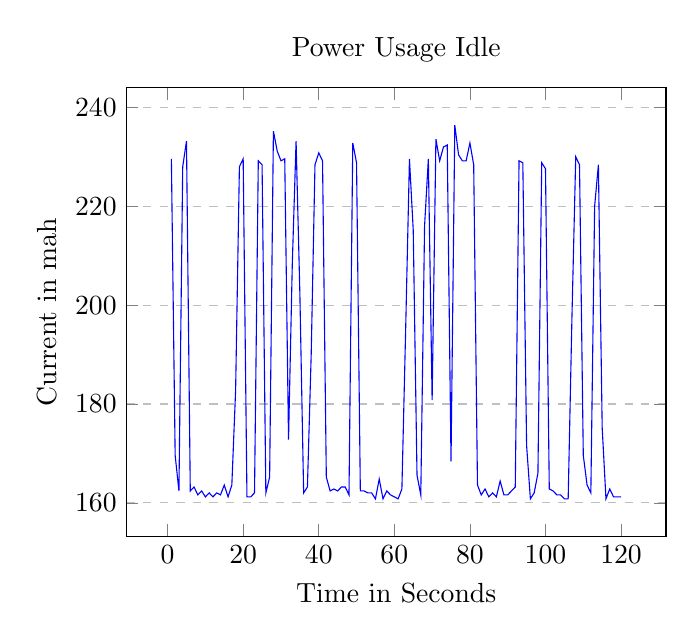
\begin{tikzpicture}
    \begin{axis}[
    title={Power Usage Idle},
    xlabel={Time in Seconds},
    ylabel={Current in mah},
    %ytick=data,
    %xtick=data,
    ymajorgrids=true,
    legend pos=outer north east,
    grid style=dashed,
    ]
    \addplot[
        color=blue,
    ]
    coordinates {
        (1,229.60)
        (2,169.60)
        (3,162.40)
        (4,228.00)
        (5,233.20)
        (6,162.40)
        (7,163.20)
        (8,161.60)
        (9,162.40)
        (10,161.20)
        (11,162.00)
        (12,161.20)
        (13,162.00)
        (14,161.60)
        (15,163.60)
        (16,161.20)
        (17,163.60)
        (18,182.80)
        (19,228.00)
        (20,229.60)
        (21,161.20)
        (22,161.20)
        (23,162.00)
        (24,229.20)
        (25,228.40)
        (26,162.00)
        (27,165.20)
        (28,235.20)
        (29,231.20)
        (30,229.20)
        (31,229.60)
        (32,172.80)
        (33,208.40)
        (34,233.20)
        (35,202.40)
        (36,162.00)
        (37,163.20)
        (38,190.00)
        (39,228.40)
        (40,230.80)
        (41,229.20)
        (42,165.20)
        (43,162.40)
        (44,162.80)
        (45,162.40)
        (46,163.20)
        (47,163.20)
        (48,161.60)
        (49,232.80)
        (50,228.80)
        (51,162.40)
        (52,162.40)
        (53,162.00)
        (54,162.00)
        (55,160.80)
        (56,164.80)
        (57,160.80)
        (58,162.40)
        (59,161.60)
        (60,161.20)
        (61,160.80)
        (62,162.80)
        (63,195.20)
        (64,229.60)
        (65,215.20)
        (66,165.60)
        (67,161.60)
        (68,216.00)
        (69,229.60)
        (70,180.80)
        (71,233.60)
        (72,229.20)
        (73,232.00)
        (74,232.40)
        (75,168.40)
        (76,236.40)
        (77,230.40)
        (78,229.20)
        (79,229.20)
        (80,232.80)
        (81,228.40)
        (82,163.60)
        (83,161.60)
        (84,162.80)
        (85,161.20)
        (86,162.00)
        (87,161.20)
        (88,164.40)
        (89,161.60)
        (90,161.60)
        (91,162.40)
        (92,163.20)
        (93,229.20)
        (94,228.80)
        (95,171.60)
        (96,160.80)
        (97,162.00)
        (98,166.00)
        (99,228.80)
        (100,227.60)
        (101,162.80)
        (102,162.40)
        (103,161.60)
        (104,161.60)
        (105,160.80)
        (106,160.80)
        (107,197.60)
        (108,230.00)
        (109,228.40)
        (110,169.60)
        (111,163.60)
        (112,162.00)
        (113,220.00)
        (114,228.40)
        (115,175.20)
        (116,160.80)
        (117,162.80)
        (118,161.20)
        (119,161.20)
        (120,161.20)
    };
    \end{axis}
\end{tikzpicture}
mean: 186.32
\end{document}

    \caption{Idle power consumption with Bluetooth, HDMI and USB enabled and disabled}
    \label{fig:idle}
\end{figure}

\section{Implementation of Energy-Aware Resource Management}
\label{sec:implementation_of_energy-aware_resource_management}

Because the CPU is the main consumer of energy in the Raspberry Pi, scaling the
voltage and frequency of the CPU to control its consumption is the most viable
approach to control total energy consumption.
%the frequency and voltage of the Raspberry Pi's ARM CPU can be scaled
%dynamically with the \texttt{cpufreq}
%subsystem\footnote{\url{https://community.arm.com/oss-platforms/w/docs/528/cpufreq-dvfs}}.

\subsection{DVFS versus \texttt{cpulimit}}

\subsection{Scaling the Output of the PV Modules}

The PV modules utilized in this version of the testbed are also distributed by
SwitchDoc Labs. They state that one panel is capable of generating a peak
current of \mbox{330 mA} at \mbox{6
V}.\footnote{\url{https://switchdoc.com/2016/06/solar-panel-comparison-sunlight-test/}}
However, even while testing under strong sunlight, the modules were only capable
of generating a third of the current that is stated. In figure \ref{fig:load} it
can be observed that four of these PV modules would roughly only be capable of
supplying the necessary current to the Raspberry Pi clocked at \mbox{400 MHz},
the lowest possible clock frequency. With this current supplied, there is no
margin for adjusting the energy consumption of the compute node to the
production of the PV modules, as the clock speed could never surpass \mbox{400
MHz}. Therefore to ensure an environment, in which the whole spectrum of energy
consumed by the compute node at different frequencies can be supplied in theory,
measured currents generated by the PV modules are multiplied by the factor
three. Since the currents are still measured and reacted to in real time, the
requirements for a testbed are still met, as presented in section
\ref{sec:testbeds_emulations_and_simulations}.

\begin{figure}
    \centering
    \documentclass{standalone}
\usepackage{pgfplots}
\pgfplotsset{compat=1.18}

\begin{document}

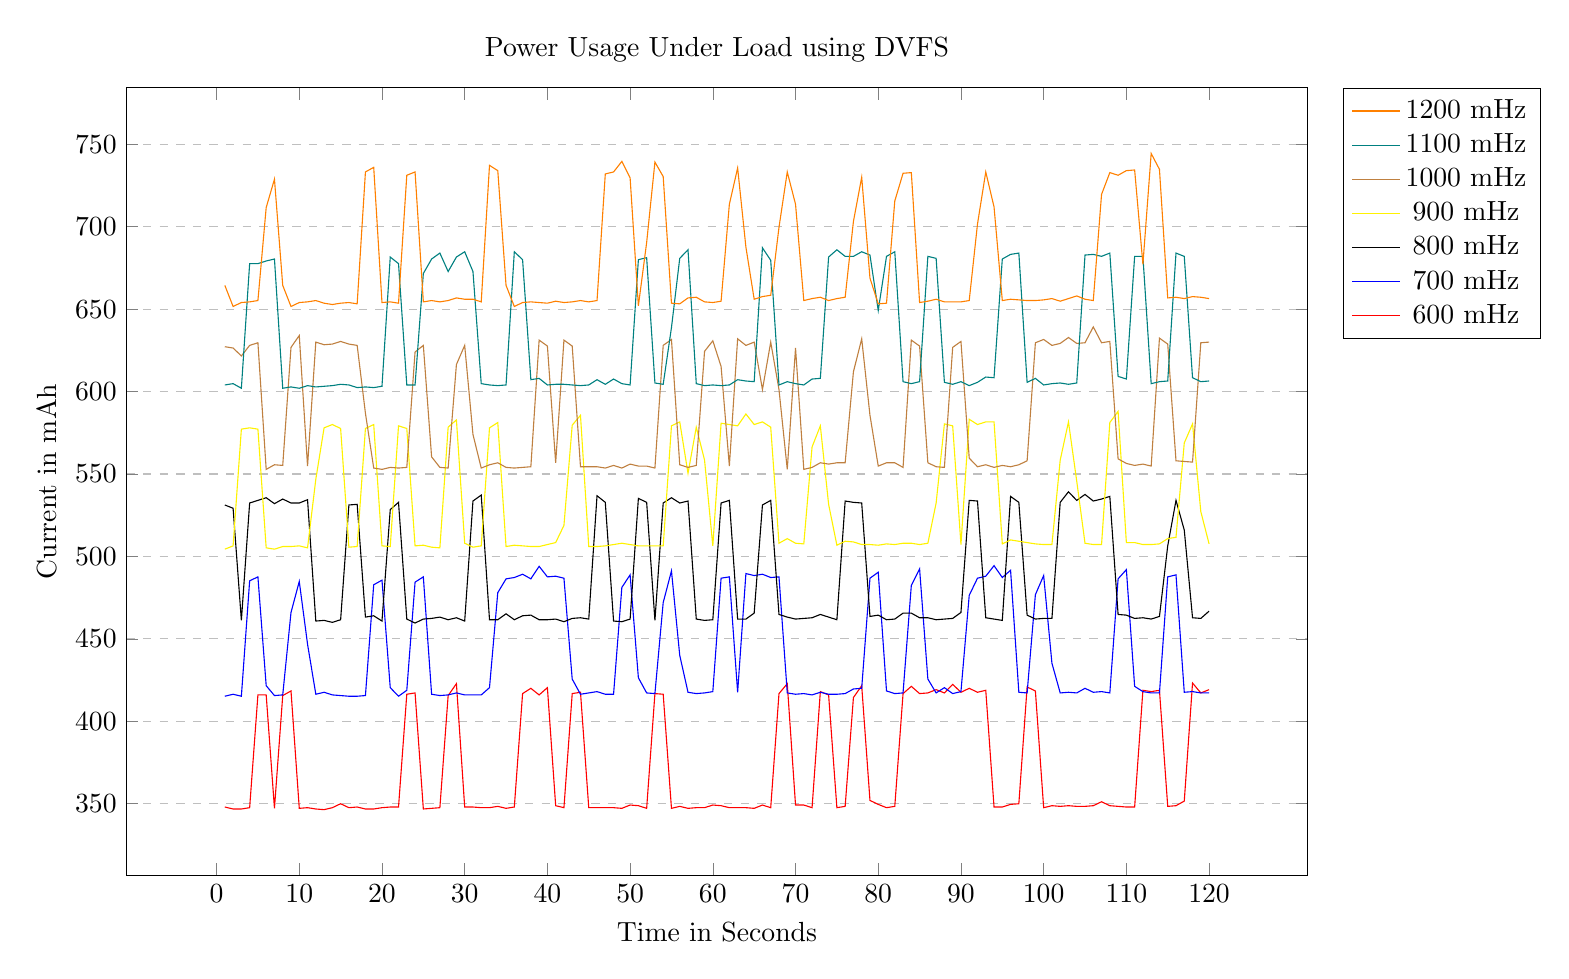
\begin{tikzpicture}
    \begin{axis}[
        title={Power Usage Under Load using DVFS},
        xlabel={Time in Seconds},
        ylabel={Current in mAh},
        %ytick=data,
        xtick={0,10,...,120},
        ymajorgrids=true,
        reverse legend,
        cycle list name=color list,
        legend pos=outer north east,
        grid style=dashed,
        height=10cm,
        width=15cm,
        scale only axis=true,
    ]
    \addplot
    coordinates {
        (1,348.00)
        (2,346.80)
        (3,346.80)
        (4,347.60)
        (5,416.00)
        (6,416.00)
        (7,347.20)
        (8,415.60)
        (9,418.40)
        (10,347.20)
        (11,347.60)
        (12,346.80)
        (13,346.40)
        (14,347.60)
        (15,350.00)
        (16,347.60)
        (17,348.00)
        (18,346.80)
        (19,346.80)
        (20,347.60)
        (21,348.00)
        (22,348.00)
        (23,416.40)
        (24,417.20)
        (25,346.80)
        (26,347.20)
        (27,347.60)
        (28,415.60)
        (29,422.80)
        (30,348.00)
        (31,348.00)
        (32,347.60)
        (33,347.60)
        (34,348.40)
        (35,347.20)
        (36,348.00)
        (37,416.80)
        (38,420.00)
        (39,416.00)
        (40,420.40)
        (41,348.80)
        (42,347.60)
        (43,416.80)
        (44,417.60)
        (45,347.60)
        (46,347.60)
        (47,347.60)
        (48,347.60)
        (49,347.20)
        (50,349.20)
        (51,348.80)
        (52,347.20)
        (53,416.80)
        (54,416.40)
        (55,347.20)
        (56,348.40)
        (57,347.20)
        (58,347.60)
        (59,347.60)
        (60,349.20)
        (61,348.80)
        (62,347.60)
        (63,347.60)
        (64,347.60)
        (65,347.20)
        (66,349.20)
        (67,347.60)
        (68,416.80)
        (69,422.80)
        (70,349.20)
        (71,349.20)
        (72,347.60)
        (73,418.00)
        (74,416.00)
        (75,347.60)
        (76,348.40)
        (77,414.40)
        (78,421.60)
        (79,352.00)
        (80,349.60)
        (81,347.60)
        (82,348.40)
        (83,416.80)
        (84,421.20)
        (85,416.80)
        (86,417.20)
        (87,419.20)
        (88,417.20)
        (89,422.40)
        (90,417.60)
        (91,420.00)
        (92,417.60)
        (93,418.80)
        (94,348.00)
        (95,348.00)
        (96,349.60)
        (97,350.00)
        (98,420.80)
        (99,418.40)
        (100,347.60)
        (101,348.80)
        (102,348.40)
        (103,348.80)
        (104,348.40)
        (105,348.40)
        (106,348.80)
        (107,351.20)
        (108,348.80)
        (109,348.40)
        (110,348.00)
        (111,348.00)
        (112,418.80)
        (113,418.00)
        (114,418.80)
        (115,348.40)
        (116,348.80)
        (117,351.60)
        (118,423.20)
        (119,417.20)
        (120,419.20)
    };
    \addlegendentry{600 mHz} % 372.07
    \addplot
    coordinates {
        (1,415.20)
        (2,416.40)
        (3,415.20)
        (4,485.20)
        (5,487.60)
        (6,421.60)
        (7,415.60)
        (8,416.00)
        (9,466.00)
        (10,484.80)
        (11,446.80)
        (12,416.40)
        (13,417.60)
        (14,416.00)
        (15,415.60)
        (16,415.20)
        (17,415.20)
        (18,415.60)
        (19,482.80)
        (20,485.60)
        (21,420.40)
        (22,415.20)
        (23,418.80)
        (24,484.40)
        (25,487.60)
        (26,416.40)
        (27,415.60)
        (28,416.00)
        (29,417.20)
        (30,416.00)
        (31,416.00)
        (32,416.00)
        (33,420.40)
        (34,478.00)
        (35,486.40)
        (36,487.20)
        (37,489.20)
        (38,486.40)
        (39,494.00)
        (40,487.60)
        (41,488.00)
        (42,486.80)
        (43,425.60)
        (44,416.40)
        (45,417.20)
        (46,418.00)
        (47,416.40)
        (48,416.40)
        (49,481.20)
        (50,488.80)
        (51,426.40)
        (52,417.20)
        (53,416.80)
        (54,472.00)
        (55,491.20)
        (56,440.00)
        (57,417.60)
        (58,416.80)
        (59,417.20)
        (60,418.00)
        (61,486.80)
        (62,487.60)
        (63,417.60)
        (64,489.60)
        (65,488.40)
        (66,489.20)
        (67,487.20)
        (68,487.60)
        (69,417.20)
        (70,416.40)
        (71,416.80)
        (72,416.00)
        (73,417.60)
        (74,416.40)
        (75,416.40)
        (76,416.80)
        (77,419.60)
        (78,420.00)
        (79,486.80)
        (80,490.40)
        (81,418.40)
        (82,416.80)
        (83,417.20)
        (84,482.40)
        (85,492.40)
        (86,425.60)
        (87,417.20)
        (88,420.40)
        (89,416.80)
        (90,418.00)
        (91,476.40)
        (92,486.80)
        (93,488.00)
        (94,494.40)
        (95,487.20)
        (96,491.60)
        (97,417.60)
        (98,417.20)
        (99,476.80)
        (100,488.40)
        (101,435.20)
        (102,417.20)
        (103,417.60)
        (104,417.20)
        (105,420.00)
        (106,417.60)
        (107,418.00)
        (108,417.20)
        (109,486.40)
        (110,492.00)
        (111,421.20)
        (112,418.00)
        (113,417.20)
        (114,417.20)
        (115,487.60)
        (116,488.80)
        (117,417.60)
        (118,418.00)
        (119,417.20)
        (120,417.20)
    };
    \addlegendentry{700 mHz} % 443.33
    \addplot
    coordinates {
        (1,531.20)
        (2,529.20)
        (3,461.20)
        (4,532.40)
        (5,534.00)
        (6,535.60)
        (7,532.00)
        (8,534.80)
        (9,532.40)
        (10,532.40)
        (11,534.40)
        (12,460.80)
        (13,461.20)
        (14,460.00)
        (15,461.60)
        (16,531.20)
        (17,531.60)
        (18,463.20)
        (19,464.00)
        (20,460.80)
        (21,528.40)
        (22,532.80)
        (23,462.00)
        (24,459.60)
        (25,462.00)
        (26,462.40)
        (27,463.20)
        (28,461.60)
        (29,462.80)
        (30,460.80)
        (31,533.60)
        (32,537.20)
        (33,461.60)
        (34,461.60)
        (35,465.20)
        (36,461.60)
        (37,464.00)
        (38,464.40)
        (39,461.60)
        (40,461.60)
        (41,462.00)
        (42,460.40)
        (43,462.40)
        (44,462.80)
        (45,462.00)
        (46,536.80)
        (47,532.80)
        (48,460.80)
        (49,460.40)
        (50,462.00)
        (51,535.20)
        (52,532.80)
        (53,461.20)
        (54,532.40)
        (55,535.60)
        (56,532.40)
        (57,533.60)
        (58,462.00)
        (59,461.20)
        (60,461.60)
        (61,532.40)
        (62,534.00)
        (63,462.00)
        (64,462.00)
        (65,465.60)
        (66,531.20)
        (67,534.00)
        (68,464.80)
        (69,463.20)
        (70,462.00)
        (71,462.40)
        (72,462.80)
        (73,464.80)
        (74,463.20)
        (75,461.60)
        (76,533.60)
        (77,532.80)
        (78,532.40)
        (79,463.60)
        (80,464.40)
        (81,461.60)
        (82,462.00)
        (83,465.60)
        (84,465.60)
        (85,462.80)
        (86,462.80)
        (87,461.60)
        (88,462.00)
        (89,462.40)
        (90,466.00)
        (91,534.00)
        (92,533.60)
        (93,462.80)
        (94,462.00)
        (95,461.20)
        (96,536.40)
        (97,532.80)
        (98,464.40)
        (99,462.00)
        (100,462.40)
        (101,462.40)
        (102,532.80)
        (103,539.20)
        (104,534.00)
        (105,537.60)
        (106,533.60)
        (107,534.80)
        (108,536.40)
        (109,464.80)
        (110,464.40)
        (111,462.40)
        (112,462.80)
        (113,462.00)
        (114,463.60)
        (115,506.40)
        (116,534.00)
        (117,516.00)
        (118,462.80)
        (119,462.40)
        (120,466.80)
    };
    \addlegendentry{800 mHz} % 488.82
    \addplot
    coordinates {
        (1,504.40)
        (2,506.40)
        (3,577.20)
        (4,578.00)
        (5,577.20)
        (6,505.20)
        (7,504.40)
        (8,506.00)
        (9,506.00)
        (10,506.40)
        (11,505.20)
        (12,546.80)
        (13,578.00)
        (14,580.00)
        (15,577.60)
        (16,505.60)
        (17,506.00)
        (18,577.60)
        (19,580.00)
        (20,506.40)
        (21,506.00)
        (22,579.20)
        (23,577.60)
        (24,506.40)
        (25,506.80)
        (26,505.60)
        (27,505.20)
        (28,578.40)
        (29,582.80)
        (30,508.00)
        (31,505.60)
        (32,506.40)
        (33,578.00)
        (34,581.20)
        (35,506.00)
        (36,506.80)
        (37,506.40)
        (38,506.00)
        (39,506.00)
        (40,507.20)
        (41,508.40)
        (42,518.80)
        (43,579.60)
        (44,585.60)
        (45,506.00)
        (46,506.00)
        (47,506.40)
        (48,507.20)
        (49,508.00)
        (50,507.20)
        (51,506.40)
        (52,506.40)
        (53,506.40)
        (54,506.40)
        (55,579.20)
        (56,581.60)
        (57,550.40)
        (58,578.40)
        (59,558.40)
        (60,506.40)
        (61,580.80)
        (62,580.00)
        (63,579.20)
        (64,586.40)
        (65,580.00)
        (66,581.60)
        (67,578.40)
        (68,508.00)
        (69,510.80)
        (70,508.00)
        (71,507.60)
        (72,566.40)
        (73,579.20)
        (74,531.60)
        (75,506.80)
        (76,509.20)
        (77,508.80)
        (78,507.20)
        (79,507.20)
        (80,506.80)
        (81,507.60)
        (82,507.20)
        (83,508.00)
        (84,508.00)
        (85,507.20)
        (86,508.00)
        (87,532.40)
        (88,580.40)
        (89,579.20)
        (90,507.20)
        (91,583.20)
        (92,580.00)
        (93,581.60)
        (94,581.60)
        (95,507.60)
        (96,510.00)
        (97,509.20)
        (98,508.40)
        (99,507.60)
        (100,507.20)
        (101,507.20)
        (102,558.40)
        (103,581.60)
        (104,545.60)
        (105,508.00)
        (106,507.20)
        (107,507.20)
        (108,581.20)
        (109,588.00)
        (110,508.40)
        (111,508.40)
        (112,507.20)
        (113,507.20)
        (114,507.60)
        (115,510.80)
        (116,511.60)
        (117,568.80)
        (118,580.40)
        (119,527.20)
        (120,507.60)
    };
    \addlegendentry{900 mHz} % 533.24
    \addplot
    coordinates {
        (1,627.20)
        (2,626.40)
        (3,621.60)
        (4,628.00)
        (5,629.60)
        (6,552.80)
        (7,555.60)
        (8,555.20)
        (9,626.80)
        (10,634.00)
        (11,554.80)
        (12,630.00)
        (13,628.40)
        (14,628.80)
        (15,630.40)
        (16,628.80)
        (17,628.00)
        (18,586.80)
        (19,553.60)
        (20,552.80)
        (21,554.00)
        (22,553.60)
        (23,554.00)
        (24,624.00)
        (25,628.00)
        (26,560.40)
        (27,554.00)
        (28,553.60)
        (29,616.40)
        (30,628.00)
        (31,574.00)
        (32,553.60)
        (33,555.60)
        (34,556.80)
        (35,554.00)
        (36,553.60)
        (37,554.00)
        (38,554.40)
        (39,631.20)
        (40,627.60)
        (41,556.80)
        (42,631.20)
        (43,627.60)
        (44,554.40)
        (45,554.40)
        (46,554.40)
        (47,553.60)
        (48,555.20)
        (49,553.60)
        (50,556.00)
        (51,554.80)
        (52,554.80)
        (53,553.60)
        (54,628.00)
        (55,631.60)
        (56,555.60)
        (57,554.00)
        (58,555.20)
        (59,624.40)
        (60,630.80)
        (61,615.20)
        (62,554.80)
        (63,632.00)
        (64,628.00)
        (65,630.00)
        (66,601.20)
        (67,630.00)
        (68,601.20)
        (69,552.80)
        (70,626.40)
        (71,552.80)
        (72,554.00)
        (73,556.80)
        (74,556.00)
        (75,556.80)
        (76,556.80)
        (77,612.00)
        (78,632.00)
        (79,585.60)
        (80,554.80)
        (81,556.80)
        (82,556.80)
        (83,554.00)
        (84,631.20)
        (85,627.60)
        (86,556.80)
        (87,554.40)
        (88,554.00)
        (89,626.80)
        (90,630.40)
        (91,559.60)
        (92,554.40)
        (93,555.60)
        (94,554.00)
        (95,555.20)
        (96,554.40)
        (97,555.60)
        (98,558.00)
        (99,629.60)
        (100,631.60)
        (101,628.00)
        (102,629.20)
        (103,632.80)
        (104,629.20)
        (105,629.60)
        (106,639.20)
        (107,629.60)
        (108,630.40)
        (109,559.20)
        (110,556.40)
        (111,555.20)
        (112,556.00)
        (113,554.80)
        (114,632.40)
        (115,628.80)
        (116,558.00)
        (117,557.60)
        (118,557.20)
        (119,629.60)
        (120,630.00)
    };
    \addlegendentry{1000 mHz} % 587.75
    \addplot
    coordinates {
        (1,604.00)
        (2,604.80)
        (3,602.00)
        (4,677.60)
        (5,677.60)
        (6,679.20)
        (7,680.40)
        (8,602.00)
        (9,602.80)
        (10,602.00)
        (11,603.60)
        (12,602.80)
        (13,603.20)
        (14,603.60)
        (15,604.40)
        (16,604.00)
        (17,602.40)
        (18,602.80)
        (19,602.40)
        (20,603.20)
        (21,681.60)
        (22,677.60)
        (23,604.00)
        (24,604.00)
        (25,671.60)
        (26,680.40)
        (27,684.00)
        (28,672.80)
        (29,681.60)
        (30,684.80)
        (31,672.80)
        (32,604.80)
        (33,604.00)
        (34,603.60)
        (35,604.00)
        (36,684.80)
        (37,680.00)
        (38,607.20)
        (39,608.00)
        (40,604.00)
        (41,604.40)
        (42,604.40)
        (43,604.00)
        (44,603.60)
        (45,604.00)
        (46,607.20)
        (47,604.40)
        (48,607.60)
        (49,604.80)
        (50,604.00)
        (51,680.00)
        (52,681.20)
        (53,605.20)
        (54,604.40)
        (55,638.80)
        (56,680.80)
        (57,686.00)
        (58,604.80)
        (59,603.60)
        (60,604.00)
        (61,603.60)
        (62,604.00)
        (63,607.20)
        (64,606.40)
        (65,606.00)
        (66,687.20)
        (67,679.60)
        (68,604.00)
        (69,606.00)
        (70,604.80)
        (71,604.00)
        (72,607.60)
        (73,608.00)
        (74,681.60)
        (75,686.00)
        (76,682.00)
        (77,682.00)
        (78,684.80)
        (79,682.80)
        (80,649.20)
        (81,682.00)
        (82,684.80)
        (83,606.00)
        (84,604.80)
        (85,606.00)
        (86,682.00)
        (87,680.80)
        (88,605.60)
        (89,604.40)
        (90,606.00)
        (91,603.60)
        (92,605.60)
        (93,608.80)
        (94,608.40)
        (95,680.40)
        (96,683.20)
        (97,684.00)
        (98,605.60)
        (99,608.00)
        (100,604.00)
        (101,604.80)
        (102,605.20)
        (103,604.40)
        (104,605.20)
        (105,682.80)
        (106,683.20)
        (107,682.00)
        (108,684.00)
        (109,609.20)
        (110,607.60)
        (111,682.00)
        (112,682.00)
        (113,604.80)
        (114,606.00)
        (115,606.40)
        (116,684.00)
        (117,682.00)
        (118,608.40)
        (119,606.00)
        (120,606.40)
    };
    \addlegendentry{1100 mHz} % 632.37
    \addplot
    coordinates {
        (1,664.40)
        (2,651.60)
        (3,654.00)
        (4,654.40)
        (5,655.20)
        (6,711.60)
        (7,728.80)
        (8,664.40)
        (9,651.60)
        (10,654.00)
        (11,654.40)
        (12,655.20)
        (13,653.60)
        (14,652.80)
        (15,653.60)
        (16,654.00)
        (17,653.20)
        (18,733.20)
        (19,736.00)
        (20,654.00)
        (21,654.40)
        (22,653.60)
        (23,731.20)
        (24,733.20)
        (25,654.40)
        (26,655.20)
        (27,654.40)
        (28,655.20)
        (29,656.80)
        (30,656.00)
        (31,656.00)
        (32,654.40)
        (33,737.20)
        (34,734.00)
        (35,664.40)
        (36,651.60)
        (37,654.00)
        (38,654.40)
        (39,654.00)
        (40,653.60)
        (41,654.80)
        (42,654.00)
        (43,654.40)
        (44,655.20)
        (45,654.40)
        (46,655.20)
        (47,732.00)
        (48,733.20)
        (49,739.60)
        (50,729.60)
        (51,652.00)
        (52,690.40)
        (53,739.20)
        (54,730.40)
        (55,653.60)
        (56,653.20)
        (57,656.80)
        (58,657.20)
        (59,654.40)
        (60,654.00)
        (61,654.80)
        (62,713.60)
        (63,735.60)
        (64,687.60)
        (65,656.00)
        (66,657.60)
        (67,658.40)
        (68,699.60)
        (69,733.20)
        (70,713.60)
        (71,655.20)
        (72,656.40)
        (73,657.20)
        (74,655.20)
        (75,656.40)
        (76,657.20)
        (77,703.20)
        (78,730.00)
        (79,668.80)
        (80,653.20)
        (81,653.60)
        (82,715.60)
        (83,732.40)
        (84,732.80)
        (85,654.00)
        (86,654.80)
        (87,656.00)
        (88,654.40)
        (89,654.40)
        (90,654.40)
        (91,655.20)
        (92,701.60)
        (93,733.20)
        (94,712.00)
        (95,655.20)
        (96,656.00)
        (97,655.60)
        (98,655.20)
        (99,655.20)
        (100,655.60)
        (101,656.40)
        (102,654.80)
        (103,656.40)
        (104,658.00)
        (105,656.00)
        (106,655.20)
        (107,719.60)
        (108,732.80)
        (109,731.20)
        (110,734.00)
        (111,734.40)
        (112,677.20)
        (113,744.40)
        (114,734.80)
        (115,656.80)
        (116,657.20)
        (117,656.40)
        (118,657.60)
        (119,657.20)
        (120,656.40)
    };
    \addlegendentry{1200 mHz} % 676.65
    \end{axis}
\end{tikzpicture}
\end{document}

    \caption{Power usage under load with different frequencies}
    \label{fig:load}
\end{figure}

\begin{figure}
    \centering
    \documentclass{standalone}
\usepackage{pgfplots}
\pgfplotsset{compat=1.18}

\begin{document}

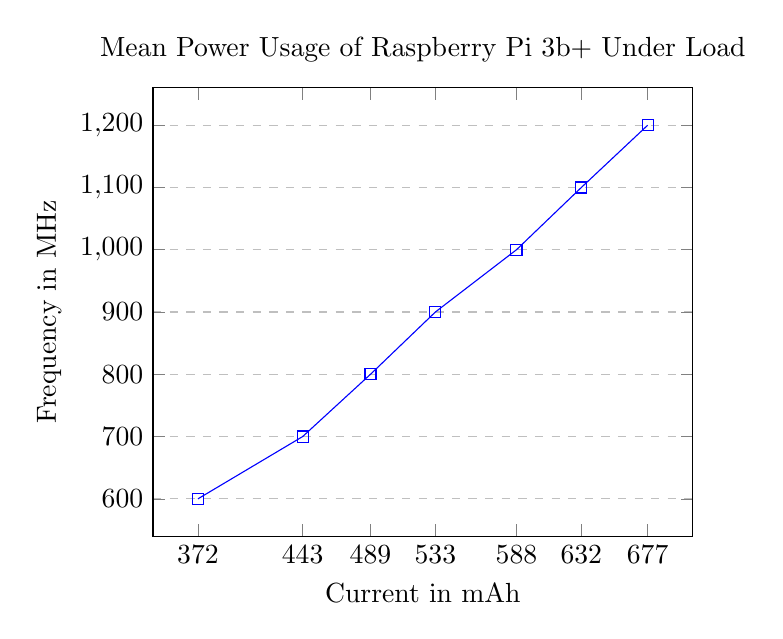
\begin{tikzpicture}
    \begin{axis}[
        title={Mean Power Usage of Raspberry Pi 3b+ Under Load},
        xlabel={Current in mAh},
        ylabel={Frequency in MHz},
        ytick=data,
        xtick=data,
        ymajorgrids=true,
        grid style=dashed,
        cycle list name=color list,
    ]
    \addplot[
        color=blue,
        mark=square,
    ]
    coordinates {
        (372,600)
        (443,700)
        (489,800)
        (533,900)
        (588,1000)
        (632,1100)
        (677,1200)
    };
    \end{axis}
\end{tikzpicture}
\hspace{.5cm}

\end{document}

    \caption{Mean power usage under load with different frequencies}
    \label{fig:mean}
\end{figure}

\subsection{The Approach}

\begin{figure}
    \centering
    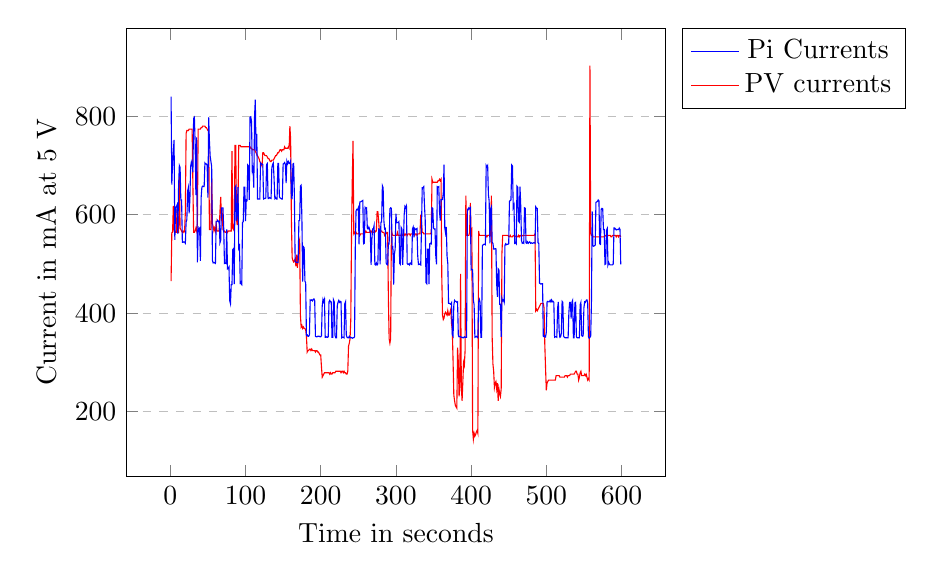
\begin{tikzpicture}
    \begin{axis}[
        xlabel={Time in seconds},
        ylabel={Current in mA at 5 V},
        %ytick=data,
        %xtick=data,
        ymajorgrids=true,
        reverse legend,
        cycle list name=color list,
        legend pos=outer north east,
        grid style=dashed,
    ]
    \addplot
    coordinates {
        (1,465)
        (2,564)
        (3,564)
        (4,618)
        (5,567)
        (6,567)
        (7,564)
        (8,564)
        (9,612)
        (10,564)
        (11,564)
        (12,678)
        (13,573)
        (14,570)
        (15,567)
        (16,564)
        (17,567)
        (18,564)
        (19,567)
        (20,606)
        (21,765)
        (22,771)
        (23,771)
        (24,771)
        (25,774)
        (26,774)
        (27,774)
        (28,774)
        (29,774)
        (30,663)
        (31,564)
        (32,564)
        (33,567)
        (34,573)
        (35,567)
        (36,582)
        (37,774)
        (38,774)
        (39,774)
        (40,774)
        (41,777)
        (42,777)
        (43,780)
        (44,780)
        (45,780)
        (46,780)
        (47,777)
        (48,777)
        (49,774)
        (50,771)
        (51,771)
        (52,570)
        (53,570)
        (54,570)
        (55,675)
        (56,582)
        (57,576)
        (58,567)
        (59,573)
        (60,567)
        (61,582)
        (62,567)
        (63,567)
        (64,567)
        (65,567)
        (66,606)
        (67,636)
        (68,594)
        (69,603)
        (70,570)
        (71,567)
        (72,567)
        (73,564)
        (74,564)
        (75,567)
        (76,564)
        (77,567)
        (78,567)
        (79,567)
        (80,567)
        (81,567)
        (82,729)
        (83,573)
        (84,570)
        (85,567)
        (86,741)
        (87,741)
        (88,591)
        (89,579)
        (90,624)
        (91,741)
        (92,741)
        (93,741)
        (94,738)
        (95,738)
        (96,738)
        (97,738)
        (98,738)
        (99,738)
        (100,738)
        (101,738)
        (102,738)
        (103,738)
        (104,738)
        (105,738)
        (106,738)
        (107,735)
        (108,735)
        (109,732)
        (110,732)
        (111,732)
        (112,732)
        (113,729)
        (114,726)
        (115,723)
        (116,720)
        (117,717)
        (118,714)
        (119,708)
        (120,705)
        (121,702)
        (122,699)
        (123,726)
        (124,726)
        (125,723)
        (126,720)
        (127,720)
        (128,720)
        (129,717)
        (130,714)
        (131,714)
        (132,711)
        (133,708)
        (134,708)
        (135,711)
        (136,711)
        (137,711)
        (138,714)
        (139,717)
        (140,720)
        (141,720)
        (142,723)
        (143,726)
        (144,726)
        (145,729)
        (146,732)
        (147,732)
        (148,729)
        (149,732)
        (150,732)
        (151,732)
        (152,738)
        (153,735)
        (154,735)
        (155,735)
        (156,735)
        (157,738)
        (158,735)
        (159,780)
        (160,753)
        (161,591)
        (162,513)
        (163,507)
        (164,504)
        (165,507)
        (166,510)
        (167,495)
        (168,519)
        (169,492)
        (170,510)
        (171,543)
        (172,549)
        (173,396)
        (174,372)
        (175,375)
        (176,369)
        (177,372)
        (178,369)
        (179,369)
        (180,366)
        (181,354)
        (182,321)
        (183,324)
        (184,324)
        (185,327)
        (186,327)
        (187,324)
        (188,327)
        (189,324)
        (190,324)
        (191,324)
        (192,324)
        (193,321)
        (194,324)
        (195,324)
        (196,321)
        (197,321)
        (198,318)
        (199,315)
        (200,315)
        (201,291)
        (202,270)
        (203,273)
        (204,276)
        (205,279)
        (206,279)
        (207,279)
        (208,279)
        (209,279)
        (210,279)
        (211,279)
        (212,276)
        (213,279)
        (214,276)
        (215,276)
        (216,279)
        (217,279)
        (218,279)
        (219,279)
        (220,282)
        (221,282)
        (222,282)
        (223,282)
        (224,282)
        (225,282)
        (226,282)
        (227,279)
        (228,282)
        (229,282)
        (230,279)
        (231,282)
        (232,279)
        (233,279)
        (234,276)
        (235,276)
        (236,282)
        (237,333)
        (238,339)
        (239,348)
        (240,387)
        (241,564)
        (242,672)
        (243,750)
        (244,561)
        (245,564)
        (246,561)
        (247,564)
        (248,561)
        (249,561)
        (250,561)
        (251,564)
        (252,558)
        (253,561)
        (254,561)
        (255,561)
        (256,561)
        (257,561)
        (258,561)
        (259,564)
        (260,567)
        (261,564)
        (262,564)
        (263,564)
        (264,564)
        (265,564)
        (266,567)
        (267,564)
        (268,567)
        (269,567)
        (270,564)
        (271,564)
        (272,564)
        (273,567)
        (274,567)
        (275,606)
        (276,606)
        (277,588)
        (278,567)
        (279,567)
        (280,567)
        (281,567)
        (282,564)
        (283,564)
        (284,564)
        (285,558)
        (286,561)
        (287,561)
        (288,564)
        (289,564)
        (290,429)
        (291,348)
        (292,339)
        (293,348)
        (294,567)
        (295,561)
        (296,558)
        (297,558)
        (298,558)
        (299,558)
        (300,558)
        (301,558)
        (302,564)
        (303,558)
        (304,558)
        (305,558)
        (306,558)
        (307,558)
        (308,561)
        (309,558)
        (310,558)
        (311,561)
        (312,558)
        (313,561)
        (314,561)
        (315,558)
        (316,561)
        (317,561)
        (318,561)
        (319,558)
        (320,561)
        (321,561)
        (322,561)
        (323,561)
        (324,561)
        (325,558)
        (326,561)
        (327,561)
        (328,558)
        (329,561)
        (330,561)
        (331,561)
        (332,561)
        (333,600)
        (334,585)
        (335,564)
        (336,564)
        (337,561)
        (338,561)
        (339,561)
        (340,561)
        (341,561)
        (342,561)
        (343,561)
        (344,561)
        (345,561)
        (346,561)
        (347,564)
        (348,672)
        (349,666)
        (350,666)
        (351,666)
        (352,666)
        (353,666)
        (354,666)
        (355,666)
        (356,669)
        (357,669)
        (358,672)
        (359,669)
        (360,672)
        (361,474)
        (362,396)
        (363,387)
        (364,390)
        (365,399)
        (366,402)
        (367,399)
        (368,396)
        (369,405)
        (370,396)
        (371,396)
        (372,402)
        (373,408)
        (374,378)
        (375,366)
        (376,303)
        (377,234)
        (378,222)
        (379,213)
        (380,210)
        (381,207)
        (382,330)
        (383,300)
        (384,231)
        (385,252)
        (386,480)
        (387,249)
        (388,222)
        (389,261)
        (390,300)
        (391,294)
        (392,324)
        (393,639)
        (394,558)
        (395,558)
        (396,558)
        (397,558)
        (398,564)
        (399,624)
        (400,561)
        (401,567)
        (402,162)
        (403,144)
        (404,156)
        (405,150)
        (406,153)
        (407,159)
        (408,162)
        (409,156)
        (410,567)
        (411,558)
        (412,558)
        (413,558)
        (414,558)
        (415,558)
        (416,558)
        (417,558)
        (418,558)
        (419,558)
        (420,558)
        (421,555)
        (422,558)
        (423,558)
        (424,558)
        (425,561)
        (426,558)
        (427,639)
        (428,351)
        (429,297)
        (430,282)
        (431,249)
        (432,258)
        (433,261)
        (434,246)
        (435,258)
        (436,222)
        (437,246)
        (438,237)
        (439,231)
        (440,246)
        (441,522)
        (442,558)
        (443,558)
        (444,558)
        (445,558)
        (446,558)
        (447,558)
        (448,558)
        (449,558)
        (450,555)
        (451,555)
        (452,558)
        (453,555)
        (454,555)
        (455,555)
        (456,558)
        (457,558)
        (458,555)
        (459,555)
        (460,558)
        (461,555)
        (462,555)
        (463,558)
        (464,555)
        (465,558)
        (466,558)
        (467,555)
        (468,558)
        (469,558)
        (470,558)
        (471,558)
        (472,558)
        (473,558)
        (474,558)
        (475,558)
        (476,558)
        (477,558)
        (478,558)
        (479,558)
        (480,558)
        (481,558)
        (482,558)
        (483,558)
        (484,558)
        (485,561)
        (486,405)
        (487,408)
        (488,405)
        (489,408)
        (490,411)
        (491,414)
        (492,417)
        (493,420)
        (494,420)
        (495,420)
        (496,420)
        (497,411)
        (498,336)
        (499,288)
        (500,243)
        (501,258)
        (502,261)
        (503,264)
        (504,264)
        (505,264)
        (506,264)
        (507,264)
        (508,264)
        (509,264)
        (510,264)
        (511,264)
        (512,264)
        (513,273)
        (514,273)
        (515,273)
        (516,273)
        (517,273)
        (518,270)
        (519,270)
        (520,270)
        (521,270)
        (522,270)
        (523,270)
        (524,270)
        (525,273)
        (526,273)
        (527,273)
        (528,270)
        (529,273)
        (530,273)
        (531,273)
        (532,276)
        (533,276)
        (534,276)
        (535,276)
        (536,276)
        (537,276)
        (538,279)
        (539,282)
        (540,282)
        (541,276)
        (542,276)
        (543,264)
        (544,270)
        (545,279)
        (546,282)
        (547,273)
        (548,273)
        (549,273)
        (550,273)
        (551,276)
        (552,273)
        (553,276)
        (554,270)
        (555,264)
        (556,267)
        (557,264)
        (558,903)
        (559,564)
        (560,558)
        (561,558)
        (562,555)
        (563,555)
        (564,555)
        (565,555)
        (566,555)
        (567,555)
        (568,555)
        (569,555)
        (570,555)
        (571,555)
        (572,555)
        (573,555)
        (574,555)
        (575,555)
        (576,555)
        (577,555)
        (578,558)
        (579,558)
        (580,555)
        (581,555)
        (582,558)
        (583,558)
        (584,558)
        (585,558)
        (586,555)
        (587,555)
        (588,558)
        (589,558)
        (590,558)
        (591,558)
        (592,558)
        (593,555)
        (594,558)
        (595,558)
        (596,555)
        (597,558)
        (598,558)
        (599,555)
    };
    \addlegendentry{PV currents}
    \addplot
        coordinates {
        (1,840)
        (2,661)
        (3,707)
        (4,728)
        (5,752)
        (6,549)
        (7,615)
        (8,616)
        (9,620)
        (10,561)
        (11,658)
        (12,700)
        (13,696)
        (14,630)
        (15,630)
        (16,544)
        (17,544)
        (18,545)
        (19,544)
        (20,542)
        (21,585)
        (22,590)
        (23,648)
        (24,655)
        (25,603)
        (26,629)
        (27,698)
        (28,707)
        (29,701)
        (30,686)
        (31,796)
        (32,798)
        (33,747)
        (34,640)
        (35,757)
        (36,503)
        (37,564)
        (38,574)
        (39,572)
        (40,506)
        (41,635)
        (42,656)
        (43,658)
        (44,657)
        (45,657)
        (46,705)
        (47,703)
        (48,703)
        (49,700)
        (50,635)
        (51,798)
        (52,750)
        (53,719)
        (54,708)
        (55,698)
        (56,507)
        (57,502)
        (58,503)
        (59,502)
        (60,501)
        (61,586)
        (62,586)
        (63,589)
        (64,586)
        (65,587)
        (66,543)
        (67,548)
        (68,614)
        (69,614)
        (70,614)
        (71,573)
        (72,501)
        (73,502)
        (74,501)
        (75,570)
        (76,490)
        (77,491)
        (78,494)
        (79,425)
        (80,419)
        (81,458)
        (82,458)
        (83,529)
        (84,531)
        (85,459)
        (86,655)
        (87,658)
        (88,588)
        (89,602)
        (90,656)
        (91,532)
        (92,536)
        (93,460)
        (94,460)
        (95,458)
        (96,584)
        (97,586)
        (98,656)
        (99,656)
        (100,587)
        (101,630)
        (102,629)
        (103,701)
        (104,699)
        (105,630)
        (106,798)
        (107,799)
        (108,789)
        (109,689)
        (110,694)
        (111,655)
        (112,799)
        (113,834)
        (114,730)
        (115,764)
        (116,632)
        (117,632)
        (118,632)
        (119,632)
        (120,705)
        (121,703)
        (122,703)
        (123,702)
        (124,632)
        (125,633)
        (126,633)
        (127,634)
        (128,702)
        (129,704)
        (130,633)
        (131,633)
        (132,635)
        (133,634)
        (134,633)
        (135,696)
        (136,702)
        (137,705)
        (138,672)
        (139,633)
        (140,635)
        (141,632)
        (142,632)
        (143,704)
        (144,704)
        (145,637)
        (146,634)
        (147,633)
        (148,632)
        (149,632)
        (150,703)
        (151,704)
        (152,706)
        (153,702)
        (154,664)
        (155,709)
        (156,704)
        (157,708)
        (158,704)
        (159,704)
        (160,709)
        (161,634)
        (162,633)
        (163,703)
        (164,704)
        (165,637)
        (166,505)
        (167,504)
        (168,503)
        (169,503)
        (170,503)
        (171,588)
        (172,588)
        (173,658)
        (174,660)
        (175,591)
        (176,464)
        (177,535)
        (178,533)
        (179,465)
        (180,462)
        (181,355)
        (182,356)
        (183,353)
        (184,353)
        (185,356)
        (186,427)
        (187,426)
        (188,427)
        (189,425)
        (190,428)
        (191,429)
        (192,425)
        (193,353)
        (194,352)
        (195,352)
        (196,353)
        (197,353)
        (198,353)
        (199,352)
        (200,352)
        (201,354)
        (202,415)
        (203,428)
        (204,423)
        (205,428)
        (206,351)
        (207,351)
        (208,352)
        (209,351)
        (210,352)
        (211,423)
        (212,426)
        (213,423)
        (214,423)
        (215,351)
        (216,351)
        (217,427)
        (218,423)
        (219,355)
        (220,350)
        (221,350)
        (222,415)
        (223,422)
        (224,426)
        (225,422)
        (226,424)
        (227,423)
        (228,350)
        (229,351)
        (230,351)
        (231,350)
        (232,419)
        (233,423)
        (234,356)
        (235,351)
        (236,350)
        (237,350)
        (238,353)
        (239,350)
        (240,351)
        (241,350)
        (242,349)
        (243,350)
        (244,350)
        (245,352)
        (246,536)
        (247,608)
        (248,611)
        (249,610)
        (250,614)
        (251,540)
        (252,626)
        (253,626)
        (254,627)
        (255,628)
        (256,629)
        (257,541)
        (258,542)
        (259,615)
        (260,613)
        (261,614)
        (262,572)
        (263,571)
        (264,575)
        (265,571)
        (266,562)
        (267,498)
        (268,549)
        (269,571)
        (270,571)
        (271,578)
        (272,499)
        (273,498)
        (274,502)
        (275,498)
        (276,500)
        (277,571)
        (278,570)
        (279,499)
        (280,585)
        (281,585)
        (282,659)
        (283,655)
        (284,588)
        (285,571)
        (286,572)
        (287,502)
        (288,499)
        (289,498)
        (290,542)
        (291,541)
        (292,612)
        (293,614)
        (294,613)
        (295,532)
        (296,534)
        (297,458)
        (298,520)
        (299,530)
        (300,602)
        (301,584)
        (302,584)
        (303,584)
        (304,586)
        (305,501)
        (306,499)
        (307,574)
        (308,571)
        (309,498)
        (310,543)
        (311,600)
        (312,617)
        (313,614)
        (314,618)
        (315,501)
        (316,499)
        (317,500)
        (318,498)
        (319,502)
        (320,500)
        (321,499)
        (322,571)
        (323,575)
        (324,554)
        (325,572)
        (326,570)
        (327,571)
        (328,572)
        (329,516)
        (330,499)
        (331,500)
        (332,499)
        (333,498)
        (334,572)
        (335,655)
        (336,655)
        (337,657)
        (338,618)
        (339,588)
        (340,462)
        (341,460)
        (342,530)
        (343,530)
        (344,459)
        (345,541)
        (346,542)
        (347,541)
        (348,614)
        (349,613)
        (350,573)
        (351,571)
        (352,571)
        (353,517)
        (354,499)
        (355,657)
        (356,656)
        (357,657)
        (358,606)
        (359,588)
        (360,631)
        (361,631)
        (362,631)
        (363,644)
        (364,702)
        (365,573)
        (366,563)
        (367,575)
        (368,516)
        (369,501)
        (370,420)
        (371,420)
        (372,419)
        (373,418)
        (374,421)
        (375,356)
        (376,353)
        (377,416)
        (378,426)
        (379,424)
        (380,424)
        (381,422)
        (382,423)
        (383,354)
        (384,352)
        (385,353)
        (386,352)
        (387,351)
        (388,351)
        (389,350)
        (390,350)
        (391,352)
        (392,351)
        (393,351)
        (394,351)
        (395,611)
        (396,610)
        (397,614)
        (398,612)
        (399,614)
        (400,488)
        (401,489)
        (402,488)
        (403,427)
        (404,417)
        (405,351)
        (406,352)
        (407,353)
        (408,351)
        (409,350)
        (410,423)
        (411,428)
        (412,422)
        (413,351)
        (414,351)
        (415,537)
        (416,539)
        (417,540)
        (418,540)
        (419,539)
        (420,700)
        (421,697)
        (422,700)
        (423,641)
        (424,628)
        (425,542)
        (426,612)
        (427,616)
        (428,544)
        (429,542)
        (430,530)
        (431,530)
        (432,531)
        (433,531)
        (434,459)
        (435,433)
        (436,490)
        (437,488)
        (438,418)
        (439,418)
        (440,352)
        (441,430)
        (442,425)
        (443,427)
        (444,422)
        (445,538)
        (446,541)
        (447,539)
        (448,540)
        (449,540)
        (450,541)
        (451,627)
        (452,629)
        (453,630)
        (454,701)
        (455,699)
        (456,615)
        (457,620)
        (458,542)
        (459,543)
        (460,541)
        (461,658)
        (462,656)
        (463,587)
        (464,585)
        (465,657)
        (466,618)
        (467,548)
        (468,542)
        (469,543)
        (470,542)
        (471,614)
        (472,613)
        (473,543)
        (474,542)
        (475,545)
        (476,542)
        (477,544)
        (478,545)
        (479,542)
        (480,543)
        (481,542)
        (482,542)
        (483,543)
        (484,543)
        (485,542)
        (486,616)
        (487,613)
        (488,613)
        (489,543)
        (490,542)
        (491,461)
        (492,460)
        (493,459)
        (494,460)
        (495,460)
        (496,353)
        (497,352)
        (498,354)
        (499,352)
        (500,361)
        (501,423)
        (502,424)
        (503,423)
        (504,423)
        (505,426)
        (506,423)
        (507,427)
        (508,423)
        (509,424)
        (510,422)
        (511,351)
        (512,352)
        (513,352)
        (514,351)
        (515,410)
        (516,423)
        (517,366)
        (518,351)
        (519,352)
        (520,359)
        (521,424)
        (522,422)
        (523,353)
        (524,351)
        (525,350)
        (526,350)
        (527,350)
        (528,350)
        (529,350)
        (530,401)
        (531,422)
        (532,422)
        (533,389)
        (534,422)
        (535,426)
        (536,350)
        (537,350)
        (538,421)
        (539,422)
        (540,352)
        (541,350)
        (542,350)
        (543,350)
        (544,350)
        (545,417)
        (546,422)
        (547,355)
        (548,353)
        (549,354)
        (550,411)
        (551,423)
        (552,422)
        (553,426)
        (554,427)
        (555,422)
        (556,352)
        (557,349)
        (558,351)
        (559,353)
        (560,420)
        (561,607)
        (562,537)
        (563,536)
        (564,537)
        (565,538)
        (566,625)
        (567,626)
        (568,627)
        (569,630)
        (570,628)
        (571,541)
        (572,540)
        (573,611)
        (574,613)
        (575,612)
        (576,570)
        (577,570)
        (578,499)
        (579,500)
        (580,568)
        (581,572)
        (582,498)
        (583,503)
        (584,499)
        (585,498)
        (586,498)
        (587,498)
        (588,498)
        (589,500)
        (590,573)
        (591,573)
        (592,571)
        (593,569)
        (594,570)
        (595,570)
        (596,570)
        (597,573)
        (598,570)
        (599,499)
        };
    \addlegendentry{Pi Currents}
    \end{axis}
\end{tikzpicture}

    \caption{aware}
    \label{fig:aware}
\end{figure}

\begin{figure}
    \centering
    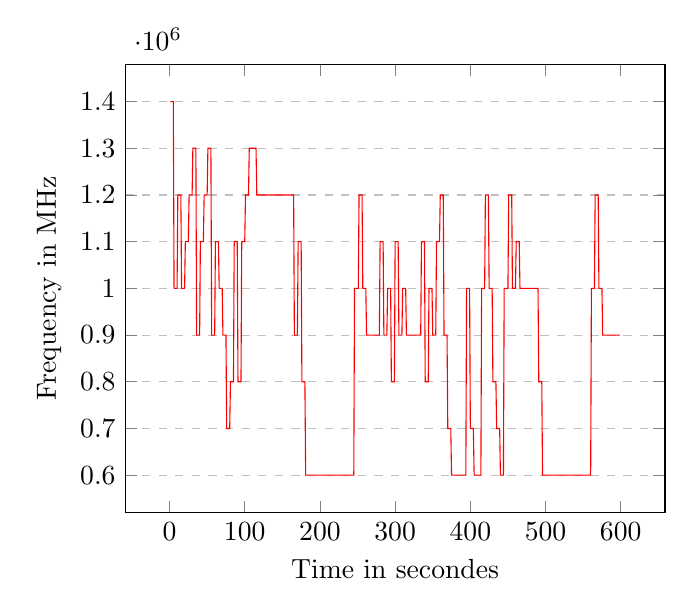
\begin{tikzpicture}
    \begin{axis}[
        xlabel={Time in secondes},
        ylabel={Frequency in MHz},
        ytick=data,
        %xtick=data,
        ymajorgrids=true,
        grid style=dashed,
        legend pos=outer north east,
        cycle list name=color list,
    ]
    \addplot
    coordinates {
        (1,1400000)
        (2,1400000)
        (3,1400000)
        (4,1400000)
        (5,1400000)
        (6,1000000)
        (7,1000000)
        (8,1000000)
        (9,1000000)
        (10,1000000)
        (11,1200000)
        (12,1200000)
        (13,1200000)
        (14,1200000)
        (15,1200000)
        (16,1000000)
        (17,1000000)
        (18,1000000)
        (19,1000000)
        (20,1000000)
        (21,1100000)
        (22,1100000)
        (23,1100000)
        (24,1100000)
        (25,1100000)
        (26,1200000)
        (27,1200000)
        (28,1200000)
        (29,1200000)
        (30,1200000)
        (31,1300000)
        (32,1300000)
        (33,1300000)
        (34,1300000)
        (35,1300000)
        (36,900000)
        (37,900000)
        (38,900000)
        (39,900000)
        (40,900000)
        (41,1100000)
        (42,1100000)
        (43,1100000)
        (44,1100000)
        (45,1100000)
        (46,1200000)
        (47,1200000)
        (48,1200000)
        (49,1200000)
        (50,1200000)
        (51,1300000)
        (52,1300000)
        (53,1300000)
        (54,1300000)
        (55,1300000)
        (56,900000)
        (57,900000)
        (58,900000)
        (59,900000)
        (60,900000)
        (61,1100000)
        (62,1100000)
        (63,1100000)
        (64,1100000)
        (65,1100000)
        (66,1000000)
        (67,1000000)
        (68,1000000)
        (69,1000000)
        (70,1000000)
        (71,900000)
        (72,900000)
        (73,900000)
        (74,900000)
        (75,900000)
        (76,700000)
        (77,700000)
        (78,700000)
        (79,700000)
        (80,700000)
        (81,800000)
        (82,800000)
        (83,800000)
        (84,800000)
        (85,800000)
        (86,1100000)
        (87,1100000)
        (88,1100000)
        (89,1100000)
        (90,1100000)
        (91,800000)
        (92,800000)
        (93,800000)
        (94,800000)
        (95,800000)
        (96,1100000)
        (97,1100000)
        (98,1100000)
        (99,1100000)
        (100,1100000)
        (101,1200000)
        (102,1200000)
        (103,1200000)
        (104,1200000)
        (105,1200000)
        (106,1300000)
        (107,1300000)
        (108,1300000)
        (109,1300000)
        (110,1300000)
        (111,1300000)
        (112,1300000)
        (113,1300000)
        (114,1300000)
        (115,1300000)
        (116,1200000)
        (117,1200000)
        (118,1200000)
        (119,1200000)
        (120,1200000)
        (121,1200000)
        (122,1200000)
        (123,1200000)
        (124,1200000)
        (125,1200000)
        (126,1200000)
        (127,1200000)
        (128,1200000)
        (129,1200000)
        (130,1200000)
        (131,1200000)
        (132,1200000)
        (133,1200000)
        (134,1200000)
        (135,1200000)
        (136,1200000)
        (137,1200000)
        (138,1200000)
        (139,1200000)
        (140,1200000)
        (141,1200000)
        (142,1200000)
        (143,1200000)
        (144,1200000)
        (145,1200000)
        (146,1200000)
        (147,1200000)
        (148,1200000)
        (149,1200000)
        (150,1200000)
        (151,1200000)
        (152,1200000)
        (153,1200000)
        (154,1200000)
        (155,1200000)
        (156,1200000)
        (157,1200000)
        (158,1200000)
        (159,1200000)
        (160,1200000)
        (161,1200000)
        (162,1200000)
        (163,1200000)
        (164,1200000)
        (165,1200000)
        (166,900000)
        (167,900000)
        (168,900000)
        (169,900000)
        (170,900000)
        (171,1100000)
        (172,1100000)
        (173,1100000)
        (174,1100000)
        (175,1100000)
        (176,800000)
        (177,800000)
        (178,800000)
        (179,800000)
        (180,800000)
        (181,600000)
        (182,600000)
        (183,600000)
        (184,600000)
        (185,600000)
        (186,600000)
        (187,600000)
        (188,600000)
        (189,600000)
        (190,600000)
        (191,600000)
        (192,600000)
        (193,600000)
        (194,600000)
        (195,600000)
        (196,600000)
        (197,600000)
        (198,600000)
        (199,600000)
        (200,600000)
        (201,600000)
        (202,600000)
        (203,600000)
        (204,600000)
        (205,600000)
        (206,600000)
        (207,600000)
        (208,600000)
        (209,600000)
        (210,600000)
        (211,600000)
        (212,600000)
        (213,600000)
        (214,600000)
        (215,600000)
        (216,600000)
        (217,600000)
        (218,600000)
        (219,600000)
        (220,600000)
        (221,600000)
        (222,600000)
        (223,600000)
        (224,600000)
        (225,600000)
        (226,600000)
        (227,600000)
        (228,600000)
        (229,600000)
        (230,600000)
        (231,600000)
        (232,600000)
        (233,600000)
        (234,600000)
        (235,600000)
        (236,600000)
        (237,600000)
        (238,600000)
        (239,600000)
        (240,600000)
        (241,600000)
        (242,600000)
        (243,600000)
        (244,600000)
        (245,600000)
        (246,1000000)
        (247,1000000)
        (248,1000000)
        (249,1000000)
        (250,1000000)
        (251,1000000)
        (252,1200000)
        (253,1200000)
        (254,1200000)
        (255,1200000)
        (256,1200000)
        (257,1000000)
        (258,1000000)
        (259,1000000)
        (260,1000000)
        (261,1000000)
        (262,900000)
        (263,900000)
        (264,900000)
        (265,900000)
        (266,900000)
        (267,900000)
        (268,900000)
        (269,900000)
        (270,900000)
        (271,900000)
        (272,900000)
        (273,900000)
        (274,900000)
        (275,900000)
        (276,900000)
        (277,900000)
        (278,900000)
        (279,900000)
        (280,1100000)
        (281,1100000)
        (282,1100000)
        (283,1100000)
        (284,1100000)
        (285,900000)
        (286,900000)
        (287,900000)
        (288,900000)
        (289,900000)
        (290,1000000)
        (291,1000000)
        (292,1000000)
        (293,1000000)
        (294,1000000)
        (295,800000)
        (296,800000)
        (297,800000)
        (298,800000)
        (299,800000)
        (300,1100000)
        (301,1100000)
        (302,1100000)
        (303,1100000)
        (304,1100000)
        (305,900000)
        (306,900000)
        (307,900000)
        (308,900000)
        (309,900000)
        (310,1000000)
        (311,1000000)
        (312,1000000)
        (313,1000000)
        (314,1000000)
        (315,900000)
        (316,900000)
        (317,900000)
        (318,900000)
        (319,900000)
        (320,900000)
        (321,900000)
        (322,900000)
        (323,900000)
        (324,900000)
        (325,900000)
        (326,900000)
        (327,900000)
        (328,900000)
        (329,900000)
        (330,900000)
        (331,900000)
        (332,900000)
        (333,900000)
        (334,900000)
        (335,1100000)
        (336,1100000)
        (337,1100000)
        (338,1100000)
        (339,1100000)
        (340,800000)
        (341,800000)
        (342,800000)
        (343,800000)
        (344,800000)
        (345,1000000)
        (346,1000000)
        (347,1000000)
        (348,1000000)
        (349,1000000)
        (350,900000)
        (351,900000)
        (352,900000)
        (353,900000)
        (354,900000)
        (355,1100000)
        (356,1100000)
        (357,1100000)
        (358,1100000)
        (359,1100000)
        (360,1200000)
        (361,1200000)
        (362,1200000)
        (363,1200000)
        (364,1200000)
        (365,900000)
        (366,900000)
        (367,900000)
        (368,900000)
        (369,900000)
        (370,700000)
        (371,700000)
        (372,700000)
        (373,700000)
        (374,700000)
        (375,600000)
        (376,600000)
        (377,600000)
        (378,600000)
        (379,600000)
        (380,600000)
        (381,600000)
        (382,600000)
        (383,600000)
        (384,600000)
        (385,600000)
        (386,600000)
        (387,600000)
        (388,600000)
        (389,600000)
        (390,600000)
        (391,600000)
        (392,600000)
        (393,600000)
        (394,600000)
        (395,1000000)
        (396,1000000)
        (397,1000000)
        (398,1000000)
        (399,1000000)
        (400,700000)
        (401,700000)
        (402,700000)
        (403,700000)
        (404,700000)
        (405,600000)
        (406,600000)
        (407,600000)
        (408,600000)
        (409,600000)
        (410,600000)
        (411,600000)
        (412,600000)
        (413,600000)
        (414,600000)
        (415,1000000)
        (416,1000000)
        (417,1000000)
        (418,1000000)
        (419,1000000)
        (420,1200000)
        (421,1200000)
        (422,1200000)
        (423,1200000)
        (424,1200000)
        (425,1000000)
        (426,1000000)
        (427,1000000)
        (428,1000000)
        (429,1000000)
        (430,800000)
        (431,800000)
        (432,800000)
        (433,800000)
        (434,800000)
        (435,700000)
        (436,700000)
        (437,700000)
        (438,700000)
        (439,700000)
        (440,600000)
        (441,600000)
        (442,600000)
        (443,600000)
        (444,600000)
        (445,1000000)
        (446,1000000)
        (447,1000000)
        (448,1000000)
        (449,1000000)
        (450,1000000)
        (451,1200000)
        (452,1200000)
        (453,1200000)
        (454,1200000)
        (455,1200000)
        (456,1000000)
        (457,1000000)
        (458,1000000)
        (459,1000000)
        (460,1000000)
        (461,1100000)
        (462,1100000)
        (463,1100000)
        (464,1100000)
        (465,1100000)
        (466,1000000)
        (467,1000000)
        (468,1000000)
        (469,1000000)
        (470,1000000)
        (471,1000000)
        (472,1000000)
        (473,1000000)
        (474,1000000)
        (475,1000000)
        (476,1000000)
        (477,1000000)
        (478,1000000)
        (479,1000000)
        (480,1000000)
        (481,1000000)
        (482,1000000)
        (483,1000000)
        (484,1000000)
        (485,1000000)
        (486,1000000)
        (487,1000000)
        (488,1000000)
        (489,1000000)
        (490,1000000)
        (491,800000)
        (492,800000)
        (493,800000)
        (494,800000)
        (495,800000)
        (496,600000)
        (497,600000)
        (498,600000)
        (499,600000)
        (500,600000)
        (501,600000)
        (502,600000)
        (503,600000)
        (504,600000)
        (505,600000)
        (506,600000)
        (507,600000)
        (508,600000)
        (509,600000)
        (510,600000)
        (511,600000)
        (512,600000)
        (513,600000)
        (514,600000)
        (515,600000)
        (516,600000)
        (517,600000)
        (518,600000)
        (519,600000)
        (520,600000)
        (521,600000)
        (522,600000)
        (523,600000)
        (524,600000)
        (525,600000)
        (526,600000)
        (527,600000)
        (528,600000)
        (529,600000)
        (530,600000)
        (531,600000)
        (532,600000)
        (533,600000)
        (534,600000)
        (535,600000)
        (536,600000)
        (537,600000)
        (538,600000)
        (539,600000)
        (540,600000)
        (541,600000)
        (542,600000)
        (543,600000)
        (544,600000)
        (545,600000)
        (546,600000)
        (547,600000)
        (548,600000)
        (549,600000)
        (550,600000)
        (551,600000)
        (552,600000)
        (553,600000)
        (554,600000)
        (555,600000)
        (556,600000)
        (557,600000)
        (558,600000)
        (559,600000)
        (560,600000)
        (561,1000000)
        (562,1000000)
        (563,1000000)
        (564,1000000)
        (565,1000000)
        (566,1200000)
        (567,1200000)
        (568,1200000)
        (569,1200000)
        (570,1200000)
        (571,1000000)
        (572,1000000)
        (573,1000000)
        (574,1000000)
        (575,1000000)
        (576,900000)
        (577,900000)
        (578,900000)
        (579,900000)
        (580,900000)
        (581,900000)
        (582,900000)
        (583,900000)
        (584,900000)
        (585,900000)
        (586,900000)
        (587,900000)
        (588,900000)
        (589,900000)
        (590,900000)
        (591,900000)
        (592,900000)
        (593,900000)
        (594,900000)
        (595,900000)
        (596,900000)
        (597,900000)
        (598,900000)
        (599,900000)
        };
    \end{axis}
\end{tikzpicture}

    \caption{aware freqs}
    \label{fig:aware_freqs}
\end{figure}
